\chapter{Evaluation and Discussion}\label{sec:evaluation}

In this chapter the reference implementation of the conceptual framework is evaluated.
At first, with the aid of three use cases it is described how a geographical visualization can create more value.
A performance analysis is conducted, to discover technical limitations and to find performance bottlenecks.
As a last step, the requirements of Chapter~\ref{sec:analysis} are used to validate the conceptual framework and the reference implementation.

\section{Use Case Scenarios}\label{sec:evaluation:use-cases}

The following three use case scenarios demonstrate how more insights can be gained with \gv{} next to the \tmap{}.

\subsection{Explain Outliers}\label{sec:evaluation:use-cases:gas-stations}

\tmaps{} can have outliers, i.e.\ unusual local maxima of a certain attribute.
If the attribute is mapped to the height of the corresponding block, a local maximum is identifiable by a block that protrudes from a group of evenly levelled blocks.
Such an example is shown in Figure~\ref{fig:evaluation:use-cases:gas-prices}.

The data set of the visualizations in the figure includes gas stations in Berlin.
The \tmap{} is configured as follows:
The layout is based on the brand name of a gas station, i.e.\ gas stations of the same brand like ``Total'' or ``Aral'' are grouped together.
Height and colour of the blocks are mapped to the price of ``Diesel'' and ``E10'' respectively.

A \tmap{} with this configuration is suited to show a correlation of brand and price.
Gas stations of brand ``Total'' are located on the center-left side of the \tmap{} and they are rather expensive in general but with smaller price variations.

This is in strong contrast to gas stations of brand ``ARAL'' in the lower left:
10 gas stations can be identified as outliers, which are more expensive than other gas stations in the group.
``Esso'' and ``Shell'', located in the center and on the lower right, show outliers, too.

Gas stations of the brands ``HEM'', ``Star'' and ``Sprint'' are generally inexpensive and located in the groups with lighter colours at the top and on the right.

However, the \tmap{} alone is not able to explain the reason for certain outliers.
What is special about the protruding blocks, i.e.\ the outliers within a group?

The \gv{} can give a possible explanation:
Many of those outliers are gas stations located next to a highway.
These gas stations are slightly more expensive in general and significantly more expensive if they belong to the brand ``ARAL''.

\begin{figure}
  \centering
  \subfloat[Tree map]{{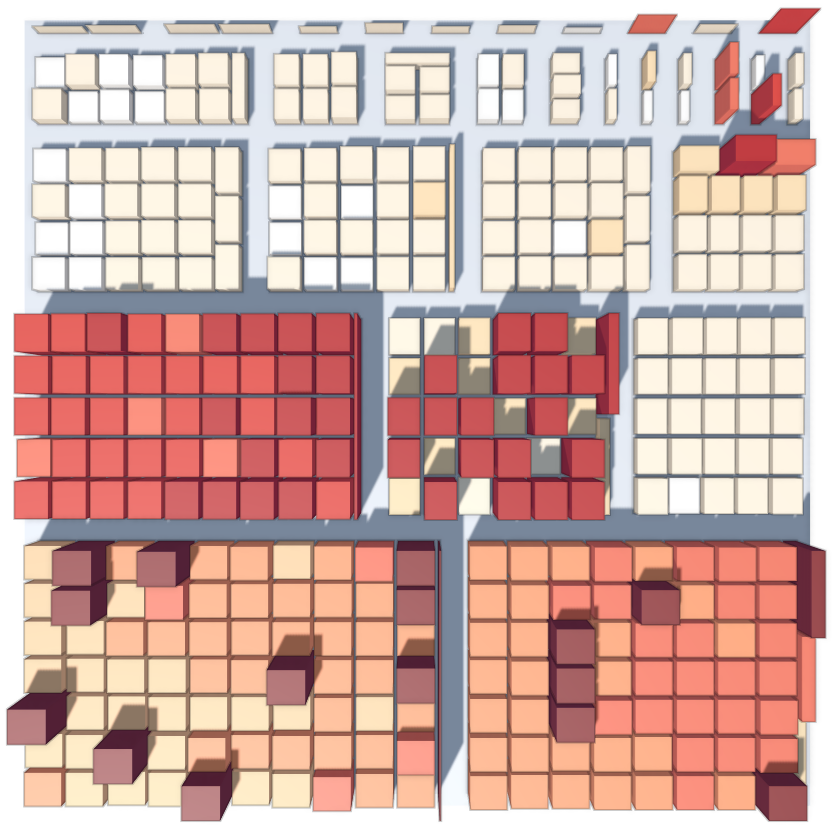
\includegraphics[width=0.4\textwidth]{figures/evaluation/use-cases/1-tmap} }}%
  \qquad
  \subfloat[Point of interest visualization]{{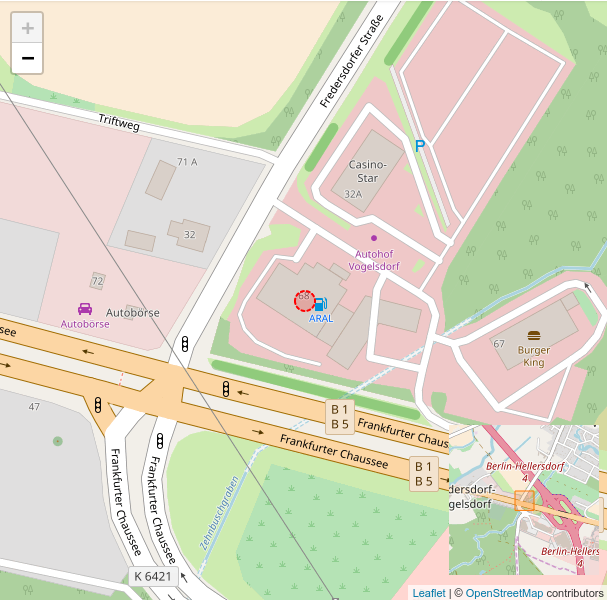
\includegraphics[width=0.4\textwidth]{figures/evaluation/use-cases/1-map} }}%
  \caption{
    Expensive gas stations, compared to other gas stations of the same brand, are often located next to highways.
  }\label{fig:evaluation:use-cases:gas-prices}
\end{figure}

\subsection{Multi-Select in the Treemap}\label{sec:evaluation:use-cases:multiselect}

This use case demonstrates the benefit of a multiple select and the ability to relate interesting features with their geographic context.
Figure~\ref{fig:evaluation:cases:multiselect:1} (a) shows a \tmap{} visualizing German constituencies with the following configuration:
The layout is based on the population density, large clusters on the right are sparsely populated districts.
Colour is based on the increase or decrease of inhabitants, a red colour indicating a growth of inhabitants.

There are three groups of items in the \tmap{} that catch our interest:
\begin{enumerate*}[label=(\arabic*)]
  \item A group of orange items on the left side of treemap,
  \item many scattered, white coloured items in the large cluster on the right and
  \item three purple coloured items in the large cluster on the right.
\end{enumerate*}

Districts in the orange group are rather densely populated and show a decline of population.
But as seen in Figure~\ref{fig:evaluation:cases:multiselect:1} (b) the districts of this group have a geographic context:
They are all located in the area of the river ``Ruhr'', a former center of the German metal processing industry.

A similar observation can be made about the white group, i.e.\ sparsely populated districts with a serious decline of population:
These districts are all located in the east of Germany, see Figure~\ref{fig:evaluation:cases:multiselect:2} (a).

And finally, even the three purple districts in the cluster of sparsely populated districts are geographically related as well:
These districts are in the vicinity of Munich, as seen in Figure~\ref{fig:evaluation:cases:multiselect:2} (b).


\begin{figure}
  \centering
  \subfloat[Tree map]{{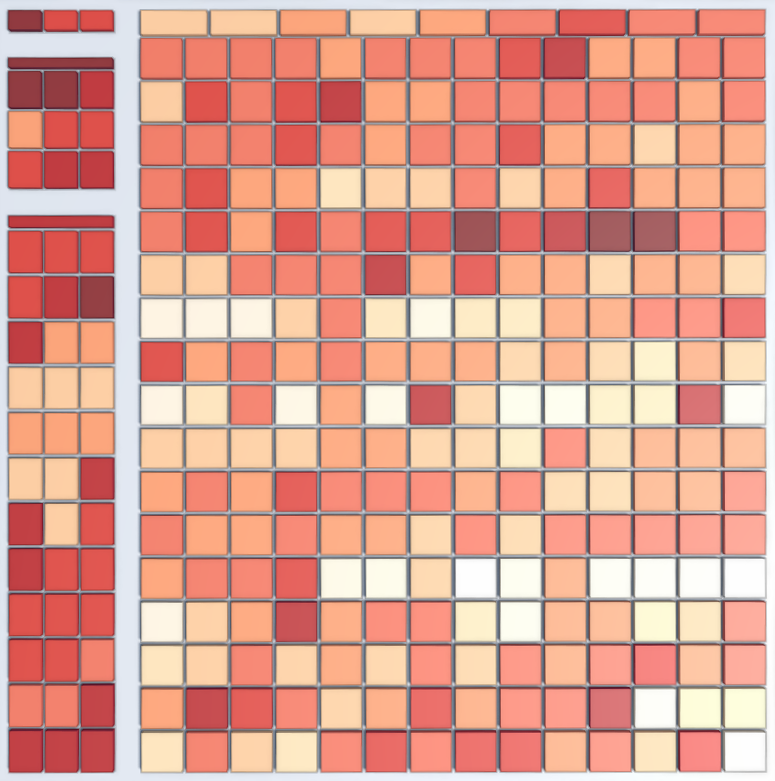
\includegraphics[width=0.4\textwidth]{figures/evaluation/use-cases/2-tmap} }}%
  \qquad
  \subfloat[Orange group]{{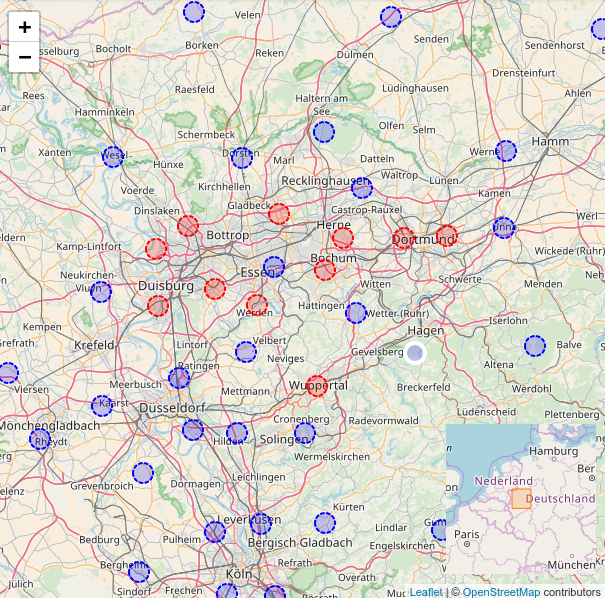
\includegraphics[width=0.4\textwidth]{figures/evaluation/use-cases/2-map-ruhr} }}%
  \caption{
    The orange coloured group on the left, districts with a moderate decline of inhabitants and large population density, are all districts of the Ruhr area.
  }\label{fig:evaluation:cases:multiselect:1}
\end{figure}

\begin{figure}
  \centering
  \subfloat[White group]{{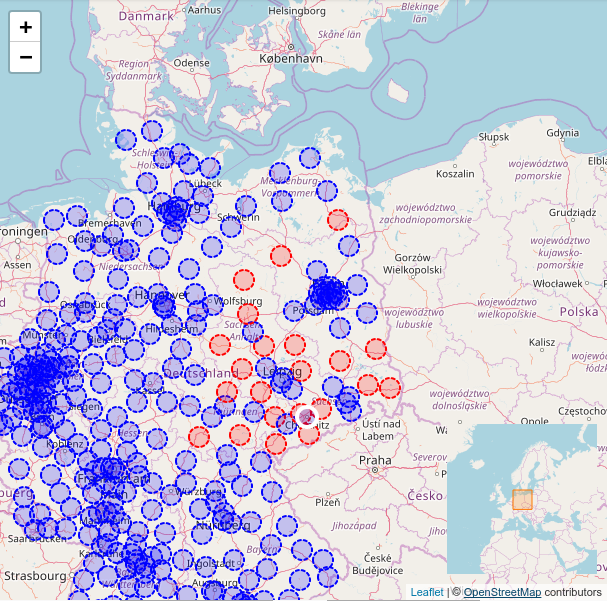
\includegraphics[width=0.4\textwidth]{figures/evaluation/use-cases/2-map-east} }}%
  \qquad
  \subfloat[Purple group]{{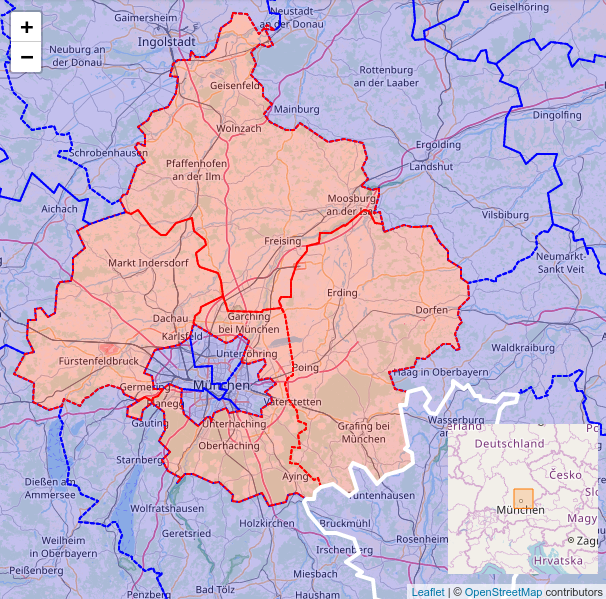
\includegraphics[width=0.4\textwidth]{figures/evaluation/use-cases/2-map-munich} }}%
  \caption{
    The sparsely populated districts with a serious decline of inhabitants are all located in the east of Germany.
    The few districts with a low population density and high increase of population are all located in the vicinity of Munich.
  }\label{fig:evaluation:cases:multiselect:2}
\end{figure}

\subsection{Bounding Box Selection in the Geographic Visualization}\label{sec:evaluation:use-cases:bounding-box}
Similar to the multiple select in Section~\ref{sec:evaluation:use-cases:multiselect}, multiple selects can be carried out by a bounding box in the \gv{}.

The layout of the \tmap{} in Figure~\ref{fig:evaluation:cases:bounding-box} (a) is based on construction activity, i.e.\ the number of completed accommodations per capita.
The colour is mapped to the increase of population.
As Berlin is known for quickly rising rents and real estate speculation, all districts in Berlin are selected with a bounding box.
All selected districts are placed in the center right group of the \tmap{}.
They are the dark red items next to the currently highlighted item in Figure~\ref{fig:evaluation:cases:bounding-box} (a).
But as seen in Figure~\ref{fig:evaluation:cases:bounding-box} (a), the districts are not in the group with the highest construction activity at the very top.

\begin{figure}
  \centering
  \subfloat[Tree map]{{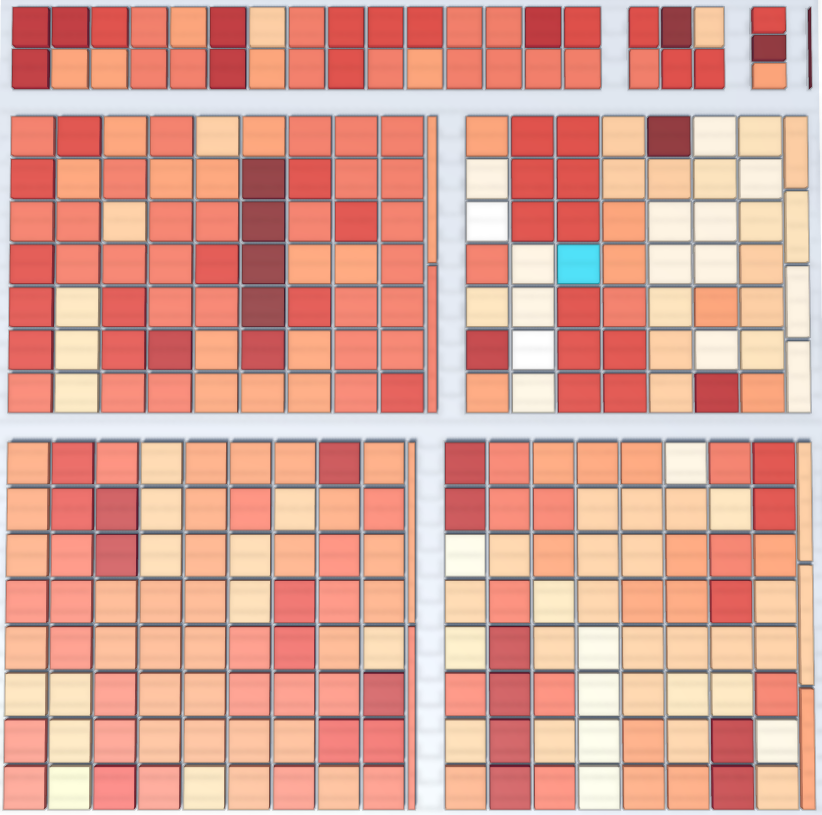
\includegraphics[width=0.4\textwidth]{figures/evaluation/use-cases/3-tmap} }}%
  \qquad
  \subfloat[Geographic map]{{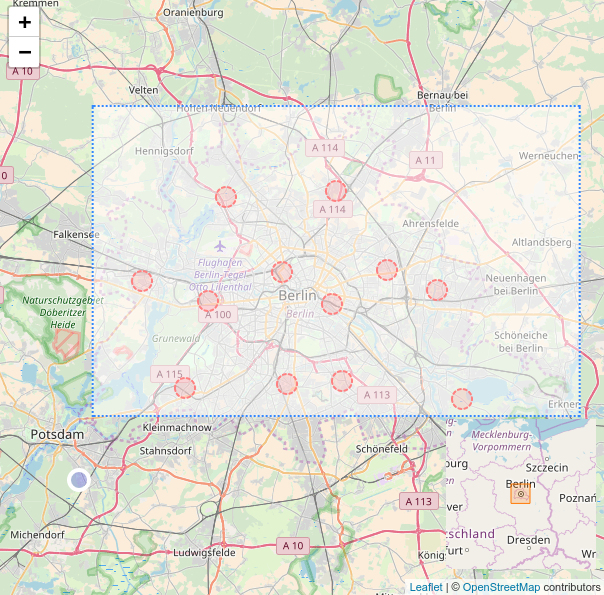
\includegraphics[width=0.4\textwidth]{figures/evaluation/use-cases/3-map} }}%
  \caption{
    A bounding box multiple select in the \gv{} can reveal a non-geographic context in the \tmap{}
  }\label{fig:evaluation:cases:bounding-box}
\end{figure}

\subsection{Use Case Summary}

The scenario in Section~\ref{sec:evaluation:use-cases:gas-stations} is a great example how a \gv{} can create more insights.
The \tmap{} alone allows to identify the outliers and also shows a possible correlation of price and brand.
However, without the \gv{} it is not possible to draw a hypothesis of the proximity to a highway being the reason for the high prices.
The geographic context is just not present in the raw data.

Deliberately selecting a particular area of interest in the \gv{} by clicking on an interesting item in the \tmap{} can be considered to be a new technique.

Similarly, in the scenario in Section~\ref{sec:evaluation:use-cases:multiselect}, the \tmap{} alone can show outliers or group of outliers.
However, it is not possible to see the geographic relation between those items in that group immediately.
The \gv{} makes the geographic context visible.
In this scenario, the multiple selection really helps to select items of the white group, which is scattered across the \tmap{}.

Finally, in the scenario of Section~\ref{sec:evaluation:use-cases:bounding-box}, the reverse is also possible:
Identify a non-geographic relation in the \tmap{} by selecting geographically related items with a bounding box.
In this case we can see a very similar construction activity.

\section{Evaluation According to Guidelines}
\textcite{Baldonado2000} introduced eight rules for multiple views.
This section checks the use case scenarios in Section~\ref{sec:evaluation:use-cases} according to these guidelines and if a positive impact on utility could be achieved.

A positive example are the rules of diversity, complementary and decomposition to improve memory and comparison~\parencite{Baldonado2000}.
Their benefits are apparent in the use case of the visualization of gas stations in Section~\ref{sec:evaluation:use-cases:gas-stations}.
The \gv{} reveals a hidden correlation, decomposes complex data into chunks and provides additional insights.
Less apparent are the benefits of the rules of self-evidence and parsimony.
In the mentioned use cases in Section~\ref{sec:evaluation:use-cases} insights are not self-evident but must be revealed with the right configuration.
Another positive example is the rule of attention management.
If the user selects one or many administrative districts in the treemap in Section~\ref{sec:evaluation:use-cases:multiselect}, the \gv{} next to it zooms on it.
In summary, the benefit of a support of learning and comparison outweighs the drawback of computational overhead.



\section{Performance Evaluation and Limitations}\label{sec:evaluation:performance}

% \todo[inline]{Das Datenset aus New York als großes Set evaluieren}
% \todo[inline]{Was ist aus den kleineren Sets geworden}

The following performance evaluation was carried out with the built-in runtime performance analysis feature of the Chrome browser.
In particular, a Chromium Browser was used in Version 62.0 (64 Bit).
The hardware specifications of the machine are listed in Table~\ref{tab:evaluation:performance:hardware}.

\begin{table}[ht]
  \centering
  \caption{Hardware specifications.}%
  \label{tab:evaluation:performance:hardware}
  \begin{tabularx}{\linewidth}{ll}
    Device name: & LENOVO ThinkPad L540 \\
    \gls{cpu} type: & Intel i3-4100M \gls{cpu} @ 2.50GHz \\
    \#\gls{cpu}s: & 4 \\
    Main memory: & 8GiB \\
    Graphics card: & Intel 4th Gen Core Processor Integrated Graphics Controller \\
  \end{tabularx}
\end{table}

A couple of data sets were used in three different scenarios:
\begin{enumerate*}[label=(\arabic*)]
  \item The \tmap{} without a geographical visualization, just publishing interactions,
  \item an example application of the geographical visualization without a \tmap{} and
  \item both visualizations together.
\end{enumerate*}

In the first and second scenario, the data set is loaded, some data points are highlighted and then some data points are focused with a single-select and a multi-select holding the control-key.
In the second scenario and third scenarios, which have a geographical visualization, many items are selected with a select box while holding the shift-key.
For every scenario there are six data sets, that is 18 profilings, and each scenario profiling took about 60 seconds to finish.

Table~\ref{tab:evaluation:performance:data-sets} shows the list of data sets used for profiling the performance of the reference implementation.
The largest data set consists of German administrative districts called ``Landkreise Deutschland'' with a total size of 2.13 MiB.
The data set with the highest number of features is called ``Immoscout Wohnungsangebote'' with 8601 coordinates German real estates, totalling 2.11 MiB.

\begin{table}[ht]
  \centering
  \caption{Data sets used for performance profiling, ordered by file size.}%
  \label{tab:evaluation:performance:data-sets}
  \begin{tabular}{lllr}
    Data Set Name & \#Features & Type & Size (MiB) \\
    \hline
    Bundesländer Deutschland      & 16   & Areas  & 0.64 \\
    Tankstellen Berlin            & 366  & Points & 0.75 \\
    Wahlkreise BT 2009            & 299  & Areas  & 0.91 \\
    Regierungsbezirke Deutschland & 31   & Areas  & 0.94 \\
    Immoscout Wohnungsangebote    & 8601 & Points & 2.11 \\
    Landkreise Deutschland        & 402  & Areas  & 2.13 \\
  \end{tabular}
\end{table}


\subsection{Immoscout}
The slowest profiling is the visualization of data set ``Immoscout''.
Chrome's runtime analysis shows a red bar at the top of the screen if the frames per second drop in such a way that it impairs the perceived interactivity.
You can see a screenshot of the analysis in Figure~\ref{fig:evaluation:performance:profiling:immoscout:fps}.


\begin{figure}[ht]
  \centering
  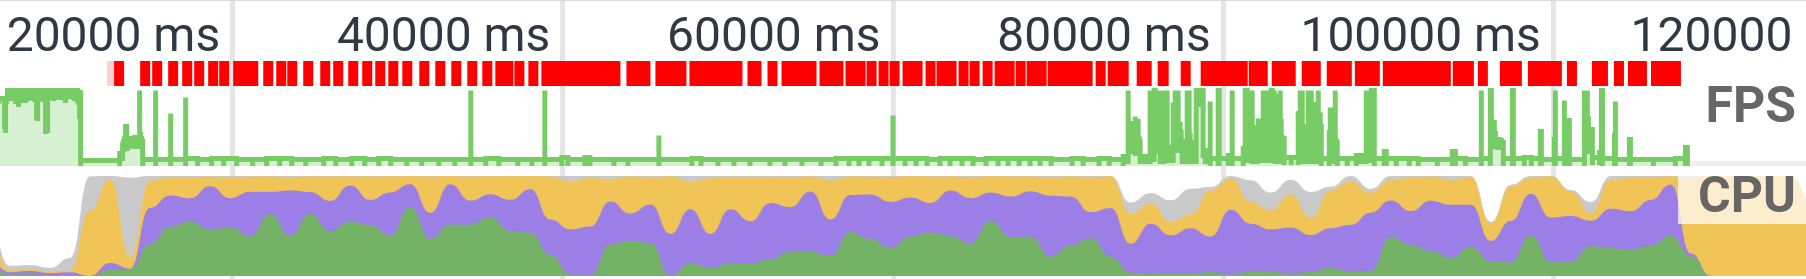
\includegraphics[width=\textwidth]{figures/evaluation/performance/profiles/immoscout_both/fps}
  \caption{During profiling of both \tmap{} and \gv{} visualizing the ``Immoscout'' data set, the frame per second rate drops to 1 FPS.}
  \label{fig:evaluation:performance:profiling:immoscout:fps}
\end{figure}

As you can see in Figure~\ref{fig:evaluation:performance:profiling:immoscout:summary} the \tmap{} spends almost the entire \gls{cpu} time in scripting.
The \gv{} has a more balanced \gls{cpu} time, spending time for painting and rendering during focusing interactions.

\begin{figure}[ht]
  \centering
  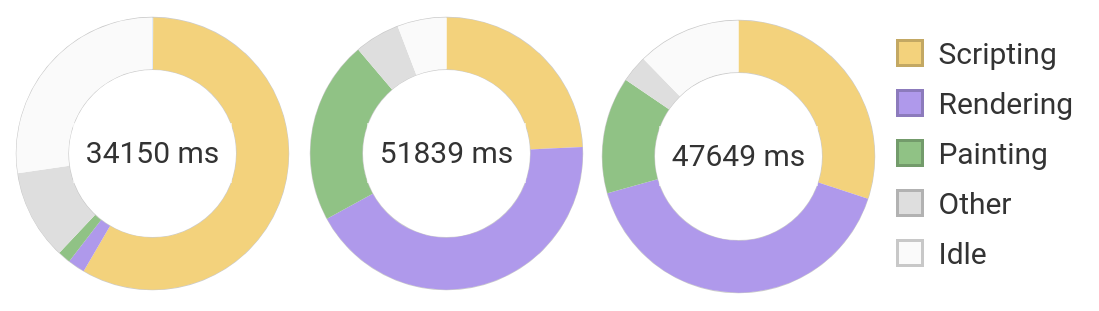
\includegraphics[width=\textwidth]{figures/evaluation/performance/summaries/immoscout}
  \caption{
    Summary of profile data for data set ``Immoscout'' of \tmap{} only (left), both \tmap{} + \gv{} (center) and only \gv{} (right).
  }\label{fig:evaluation:performance:profiling:immoscout:summary}
\end{figure}

Going through the timeline, the handling of the ``mousemove'' event can be identified to be the likely cause of this slow scripting.
The \tmap{} constantly checks the point or polygon which is under the mouse cursor.
This is likely a performance problem.

The profile summary looks totally different for the scenario of a \tmap{} along with a \gvis{}.
Compared to just a \tmap{} only, much more time is spent during painting and rendering.
This is caused by the fact, that LeafletJS moves the viewpoint and zooms if a feature is focused.
This can cause a network request and will re-render background tiles.

Note that not the communication between views hits the performance but rather the change of visual representation of views.


\begin{figure}[ht]
  \centering
  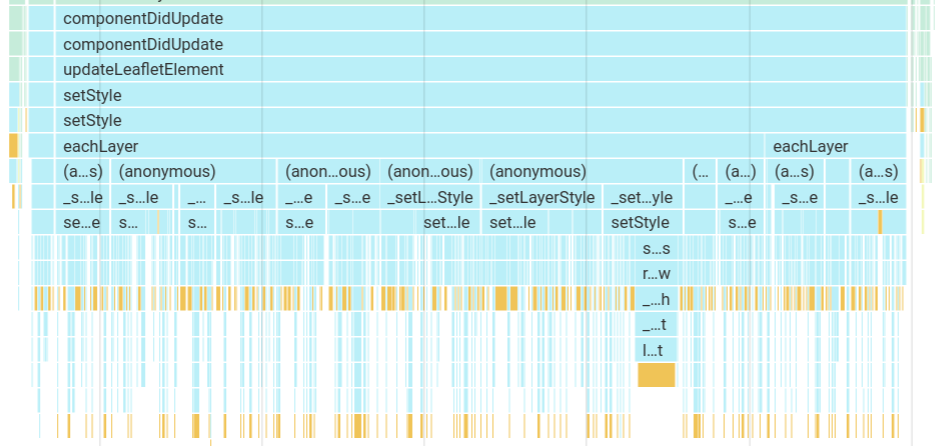
\includegraphics[width=\textwidth]{figures/evaluation/performance/profiles/immoscout_geo_only/callstack}
  \caption{
    The sawtooth pattern of the callstack during a \attr{highlight} interaction indicates an expensive iteration of all features of the \attr{GeoJSON}.
  }\label{fig:evaluation:performance:profiling:immoscout_both:callstack}
\end{figure}


Figure~\ref{fig:evaluation:performance:profiling:immoscout:fps} shows spikes whenever an interaction is made.
Most of these interactions are \attr{highlight} interactions, when the user moves the mouse cursor.
Figure~\ref{fig:evaluation:performance:profiling:immoscout_both:callstack} shows the lower part of the callstack during such a \attr{highlight} interaction.

The dominating subroutine is identified as \attr{setStyle} which spans almost the entire callstack.
Below this subroutine, you can see a lot of quick calls for each layer.
\attr{LeafletJS} iterates through all geographic features in order to update the style, e.g.\ change the stroke width.
Therefore, \attr{setStyle} seems to be costly operation for a large number of features.
This would explain why many small features have a stronger performance impact than fewer but larger features.


\subsection{Landkreise}
The profiling of data set ``Landkreise'' seems to support that assumption.
This data set is larger than ``Immoscout'' but has fewer features.
Nevertheless, the frame per second rate rarely drops in a way which has an impact on interactivity, as you can see in Figure~\ref{fig:evaluation:performance:profiling:landkreise_both:fps}.


\begin{figure}[ht]
  \centering
  \caption{
    Larger but fewer features seem to have positive effects on the frame rate.
  }\label{fig:evaluation:performance:profiling:landkreise_both:fps}
  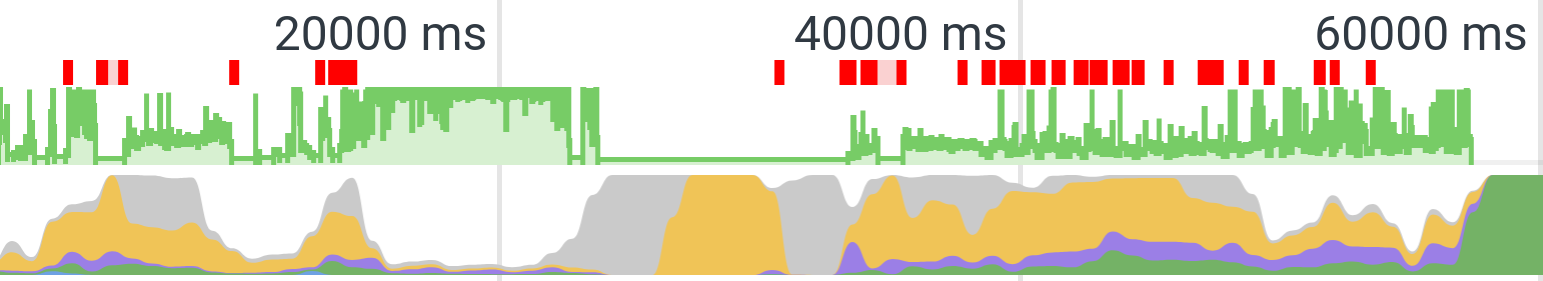
\includegraphics[width=\textwidth]{figures/evaluation/performance/profiles/landkreise_both/fps}
\end{figure}

The \gv{} alone idles almost 50\% of the \gls{cpu} time, as you can see on the right side of Figure~\ref{fig:evaluation:performance:profiling:landkreise:summary}.
\begin{figure}[ht]
  \centering
  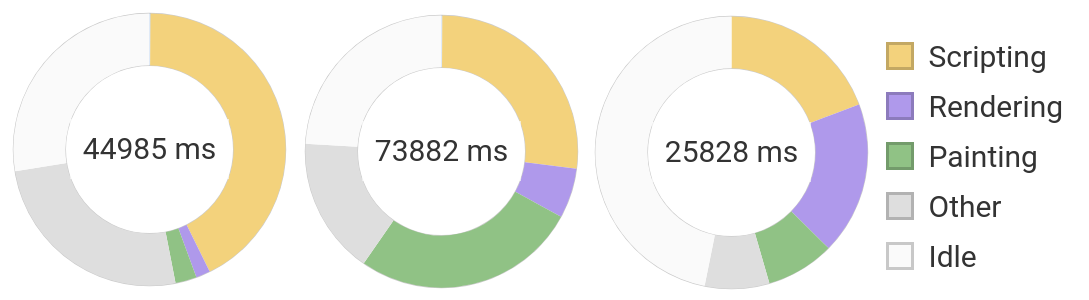
\includegraphics[width=\textwidth]{figures/evaluation/performance/summaries/landkreise}
  \caption{
    Summary of profile data for data set ``Landkreise'' of \tmap{} only (left), both \tmap{} + \gv{} (center) and only \gv{} (right).
  }\label{fig:evaluation:performance:profiling:landkreise:summary}
\end{figure}



\section{Discussion of Requirements}\label{sec:evaluation:requirements}
In this section, the reference implementation is evaluated based on the requirements from Section~\ref{sec:analysis:requirements}.

\textbf{Serialization} of interactions depends on the serialization of the published message $(M,C,P)$ as defined in Chapter~\ref{sec:concept}.
The interaction category and purpose are just strings and therefore trivial to serialize, as shown in Section~\ref{sec:implementation:concept:translation:subject-purpose}.
The interaction subject, however, can be an arbitrary JavaScript object.
The estimated size and data type of that object determines how graciously a message can be serialized.

In our case, the largest JavaScript object that is transmitted between views are geometries during initialization.
The largest data set in Table~\ref{tab:evaluation:performance:data-sets} is called ``Immoscout Wohnungsangebote'' with a file size of 2.1 MiB.
Geometries and meta data serialize well in form of GeoJSON.
The performance analysis in Section~\ref{sec:evaluation:performance} does not indicate a large impact during initialization.
Apparently, geometries seem not to be the bottleneck.

Instead, the analysis shows a performance impact for very frequent interactions, e.g.\ highlighting of entities.
Yet, the interaction subject is a list of a few ids, in most cases just one, and is therefore easy to serialize with a small resulting size.
The impact on performance is caused rather by data sets with a high number of features.

As an alternative to explicitly specifying the interaction subject, a interaction subject can be specified as a function.
The serialization of functions in JavaScript is straightforward:
They can be serialized with \attr{toString()} and deserialized with \attr{eval}.

\begin{enumerate}
\item Reversibility

Reversibility is connected to the serialization of interaction messages, too.
The undoing of an interaction needs to be implemented in each view separately.
If the interaction framework is used to publish an \attr{undo} interaction, there are two possible implementations:
\begin{enumerate*}[label=(\arabic*)]
  \item
    Each subscribed view keeps a record of every received interaction in the past and can replay these interactions up to the desired step
    \item
    if the effect of the interaction is reversible, e.g.\ the inverse of a function exists, the inverse of a function is published.
\end{enumerate*}
Both options have an undesired impact on the required memory, because a record of published messages needs to be kept in memory.
If that record is long, it will take a long time to replay every interaction up to the desired step.
As a result, reversibility is non-trivial to implement and has a potential performance impact.

\item Extensibility

The \cmv{} system is designed for loose coupling, independent views and almost no shared state.
It is lightweight and has a low complexity.
The downside of this approach is that it does not come with a huge simplification of the implementation effort in individual views.
Therefore, the system is very extensible and scales well, but the development effort for each interaction remains high.\\\\


\item Maintainability

Maintainability as described in Section~\ref{sec:analysis:requirements} means how much other parts of the code are impacted by an interaction and how error-prone the framework is.
The framework benefits of the main advantages of the publish-subscribe pattern, i.e.\ loose coupling and scalability.
On the other hand, it suffers from the main disadvantages of this software pattern, the decoupling of publisher and subscriber.
Therefore, a proper debugging of all components in the whole system is necessary.
Nevertheless, each view in the \cmv{} system has small dependencies and is therefore easy to maintain and test.

\end{enumerate}
